\begin{lstlisting}
习题2.1第1,3,4,5,6,9,10,13题
\end{lstlisting}
\begin{figure}[H]
\centering
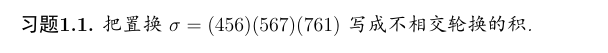
\includegraphics[width=\textwidth]{hw4-2025033113.png}
% \caption{}
\label{}
\end{figure}
\[
\sigma=(456)(567)(761)=(54)(56)(65)(67)(67)(61)=(16)(45)
\]
\begin{figure}[H]
\centering
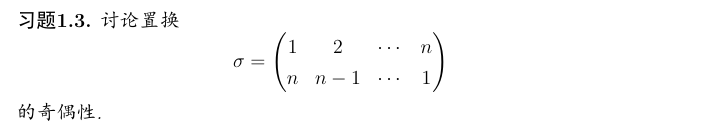
\includegraphics[width=\textwidth]{1-hw4-2025033113.png}
% \caption{}
\label{}
\end{figure}

If $n=2m$ then
\[
\sigma=(1\quad 2m)(2\quad 2m-1)\dots(m\quad m+1)
\]
The number of transpositions in the factorization is $m$. If $2|m$ then $\sigma$ is even. If $2\nmid m$ then $\sigma$ is odd.

If $n=2m-1$ then
\[
\sigma=(1\quad 2m-1)(2\quad 2m-2)\dots(m-1\quad m+1)
\]
The number of transposition in the factorization is $m-1$. If $2|m$ then $\sigma$ is odd. If $2\nmid m$ then $\sigma$ is even.

Therefore, if $n\equiv1,2(\mathrm{mod}4)$, $\sigma$ is odd. If $n\equiv0,3(\mathrm{mod}4)$, $\sigma$ is even.

\begin{figure}[H]
\centering
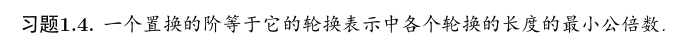
\includegraphics[width=\textwidth]{2-hw4-2025033113.png}
% \caption{}
\label{}
\end{figure}

Suppose that a permutation can be decomposed into $r$ disjoint cycles
\[
\sigma=\sigma_1\circ \sigma_2\circ \dots \circ \sigma_{r}
\]
Each $\sigma _k$ has length $a_k$, then $\lvert \sigma _k \rvert=a_k$. Therefore $\lvert \sigma \rvert|\mathrm{lcm}(a_1,\dots,a_{r})$. By the definition of $\lvert \sigma \rvert$, we have
\[
\sigma_1^{\lvert \sigma \rvert }\circ \sigma_2^{\lvert \sigma \rvert }\circ \dots \circ \sigma_{r}^{\lvert \sigma \rvert }=e
\]
Therefore $a_k|\lvert \sigma \rvert$ for each $k$. Thus $\mathrm{lcm}(a_1,\dots,a_{r})|\lvert \sigma \rvert$. Hence
\[
\lvert \sigma \rvert =\mathrm{lcm}(a_1,\dots,a_r)
\]
\begin{figure}[H]
\centering
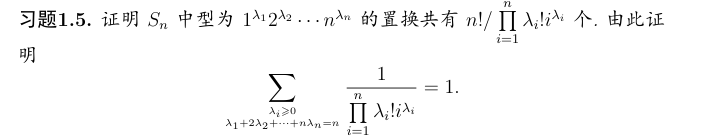
\includegraphics[width=\textwidth]{3-hw4-2025033113.png}
% \caption{}
\label{}
\end{figure}

先证明 $S_n$ 中型为 $1^{\lambda_1}2^{\lambda_2}\dots n^{\lambda _n}$ 的置换共有 $n!/\prod_{i=1}^{n}\lambda _i!i^{\lambda _i}$ 个. 我们进行如下操作:先将 $1,2,\dots,n$ 分到 $\sum_{i=1}^{n}\lambda _i$ 个盒子中:
\[
\{ 1,2,\dots,n \}\longrightarrow \overbrace{ \{ \underbrace{ . }_{ 1\text{ item} } \},\dots,\{ \underbrace{ . }_{ 1\text{ item} } \} }^{ \lambda_1\text{ items} },\{ .. \},\dots,\{ .. \},\dots,\{ \dots \}
\]
然后无视这些盒子的次序,再考虑每个盒子内元素的对应关系,比如对于有 $r$ 个元素的盒子,要求
\[
\begin{pmatrix}
a_1 & a_2 & \dots & a_{r} \\
a_{p_1} & a_{p_2} & \dots & a_{p_{r}}
\end{pmatrix}
\]
先从 $a_1$ 开始考虑,$a_{p_1}$ 的选取有 $r-1$ 种($a_{p_1}\neq a_1$),$a_{p_2}$ 的选取有 $r-2$ 种... 于是一共有 $(r-1)!$ 种.

按照上述逻辑考虑置换的种类可以知道, $S_n$ 中型为 $1^{\lambda_1}2^{\lambda_2}\dots n^{\lambda _n}$ 的置换共有
\[
\frac{n!}{\prod_{i=1}^{n} (i!)^{\lambda _i}}\cdot\frac{1}{\prod_{i=1}^{n} \lambda _i!}\cdot \prod_{i=1}^{n} ((i-1)!)^{\lambda _i}=\frac{n!}{\prod_{i=1}^{n} \lambda _i!\cdot i^{\lambda _i}}
\]
同时我们考虑 $S_n$ 的所有置换,按照 $1^{\lambda_1}2^{\lambda_2}\dots n^{\lambda _n}$ 分类计算可得
\[
n!=\sum_{\substack{\lambda _i\geq 0
\\
\lambda_1+2\lambda_2+\dots+n\lambda _n=n}}\frac{n!}{\prod_{i=1}^{n} \lambda _i!i^{\lambda _i}}
\]
于是
\[
\sum_{\substack{\lambda_i \geqslant 0 \\ \lambda_1+2 \lambda_2+\cdots+n \lambda_n=n}} \frac{1}{\prod_{i=1}^n \lambda_{i}!i^{\lambda_i}}=1 .
\]
\begin{figure}[H]
\centering
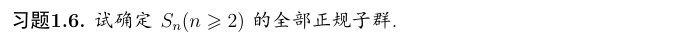
\includegraphics[width=\textwidth]{4-hw4-2025033113.png}
% \caption{}
\label{}
\end{figure}

\begin{lemma}
$A_n$ ($n>=5$) 非单.\label{c6e538}
\end{lemma}

\begin{proof}
\href{https://kconrad.math.uconn.edu/blurbs/grouptheory/Ansimple.pdf}{Ansimple.pdf}
\end{proof}

\begin{lemma}
$A_n\lhd S_n$.
\end{lemma}
\begin{proof}
Any permutation can decomposite to product of transformations. $A_n$ is defined to be the permutations in $S_n$ with even numbers of transformations in its decomposition. $A_n$ is the kernel of
\[
\phi:S_n\to \{ \pm1 \}\qquad \tau=(i_1 j_1)\dots(i_n j_n)\mapsto(-1)^{n}
\]
Thus $A_n=\ker (\phi)\lhd S_n$.
\end{proof}

$n>1,n\neq4$ 时,$S_n$ 的全部正规子群为 $S_n,A_n,\{ e \}$.

When $n=4$, evaluate all the normal subgroups of $A_4$.
\[
A_4=\{ e,(123),(132),(124),(142),(134),(143),(234),(243),(12)(34),(13)(24),(14)(23) \}
\]
$\lvert A_4 \rvert=12=2^{2}\times3$. There are 4 sylow 3-subgroups of $A_4$:
\[
\left< 123 \right> ,\left< 124 \right> ,\left< 134 \right> ,\left< 234 \right>
\]
Thus is not normal in $A_4$. There is only one sylow 2-subgroup of $A_4$:
\[
K_4\coloneqq \{ e, (12)(34),(13)(24),(14)(23)\}
\]
Thus is normal in $A_4$. C'est clair $K_4$ is simple.

$S_4$ 的全部正规子群为 $A_4,K_4,\{ e \},S_4$.
\begin{figure}[H]
\centering
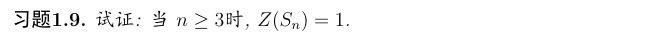
\includegraphics[width=\textwidth]{5-hw4-2025033113.png}
% \caption{}
\label{}
\end{figure}
\[
Z(S_n)\coloneqq \{ g\in G:ghg^{-1}=h,\forall h\in S_n \}
\]
Since $A_n\subseteq S_n$,
\[
Z(S_n)\subseteq Z(A_n)\lhd A_n
\]
When $n\neq4$, the simplicity and noncommutativity of $A_n$ \cref{c6e538}  implies $Z(A_n)=1$ thus $Z(S_n)=1$. When $n=4$, $Z(S_4)$ maybe $A_4,K_4$ or $1$. Since
\[
(13)\cdot(12)(34)\cdot(13)^{-1}=(14)(23)\neq (12)(34)
\]
Then $Z(S_4)$ is trivial.

\begin{figure}[H]
\centering
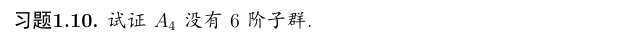
\includegraphics[width=\textwidth]{6-hw4-2025033113.png}
% \caption{}
\label{}
\end{figure}

\begin{figure}[H]
\centering
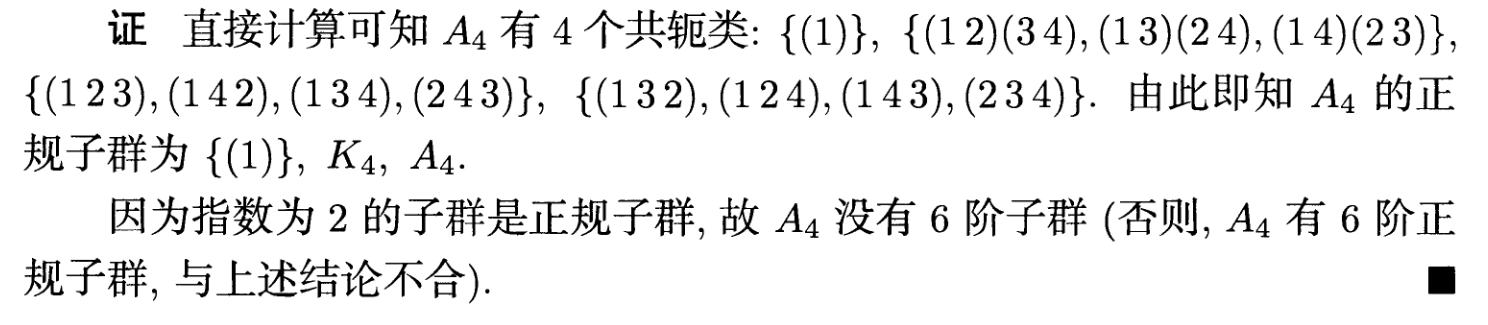
\includegraphics[width=\textwidth]{hw4-2025040100.png}
% \caption{}
\label{}
\end{figure}

\begin{figure}[H]
\centering
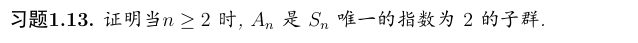
\includegraphics[width=\textwidth]{7-hw4-2025033113.png}
% \caption{}
\label{}
\end{figure}

由于指数为 2 的子群必然是正规子群,而且 $n\neq4$ 时 $S_n$ 的非平凡正规子群只有交错群 $A_n$,$n=4$ 时,$S_4$ 的非平凡正规子群只有 $A_4$ 和 $K_4$. 故得证!
